\section{\emph{Configurable Sensor} MAC ou CS-MAC}

O algoritmo desenvolvido nesse trabalho foi batizado de \emph{Configurable Sensor} MAC ou \emph{Sensor}-MAC configurável pois tem como base o algoritmo S-MAC descrito em \citeauthoronline{ye04} (\citeyear{ye04}). Conforme apresentado na seção ~\ref{sec:smac}, o protocolo S-MAC faz com que cada nó em uma vizinhança siga um mesmo cronograma que determina seus períodos de atividade e inatividade. Com isso, cada nó que deseja transmitir pacotes poderá fazê-lo no momento em que iniciar seu ciclo de atividades sem a necessidade do uso de longos preâmbulos pois o nó receptor iniciará seu ciclo de atividades no mesmo momento.

O protocolo CS-MAC possui os mesmos mecanismos de funcionamento do protocolo S-MAC, podendo ser então considerado uma extensão desse protocolo, pois adiciona a ele mecanismos que permitem que seu funcionamento e configurações sejam alterados por outras camadas da pilha de protocolo, no caso deste trabalho, pela camada de aplicação (Seção ~\ref{sec:applicationLayer}). 

Basicamente, os mecanismos de configuração implementados no protocolo CS-MAC permitem que outra camada possa determinar que o nó siga um cronograma de funcionamento arbitrário especificado por ela com qualquer finalidade. Para o teste dos mecanismos implementados no protocolo CS-MAC, foram implementados na camada de aplicação algoritmos capazes de construir uma ``via de acesso rápido'' (\emph{backbone}), por onde os pacotes poderiam trafegar mais rapidamente.

De forma simplificada, os algoritmos implementados são capazes de determinar que uma cadeia de nós situados a uma determinada distância do centro da rede (Figura ~\ref{fig:circularBackbone}) de sensores seja sincronizada de uma maneira tal que, dados os nós A, B e C pertencentes a estrutura, o tempo de transmissão de um pacote de A para C passando por B seria de aproximadamente $2 \cdot T_A$  ($1 \cdot T_A$ = transmissão de A para B, $1 \cdot T_A$ = transmissão B para C) sendo $T_A$ a duração do período de atividade de um nó. 

\begin{figure}[!htb]
\centering
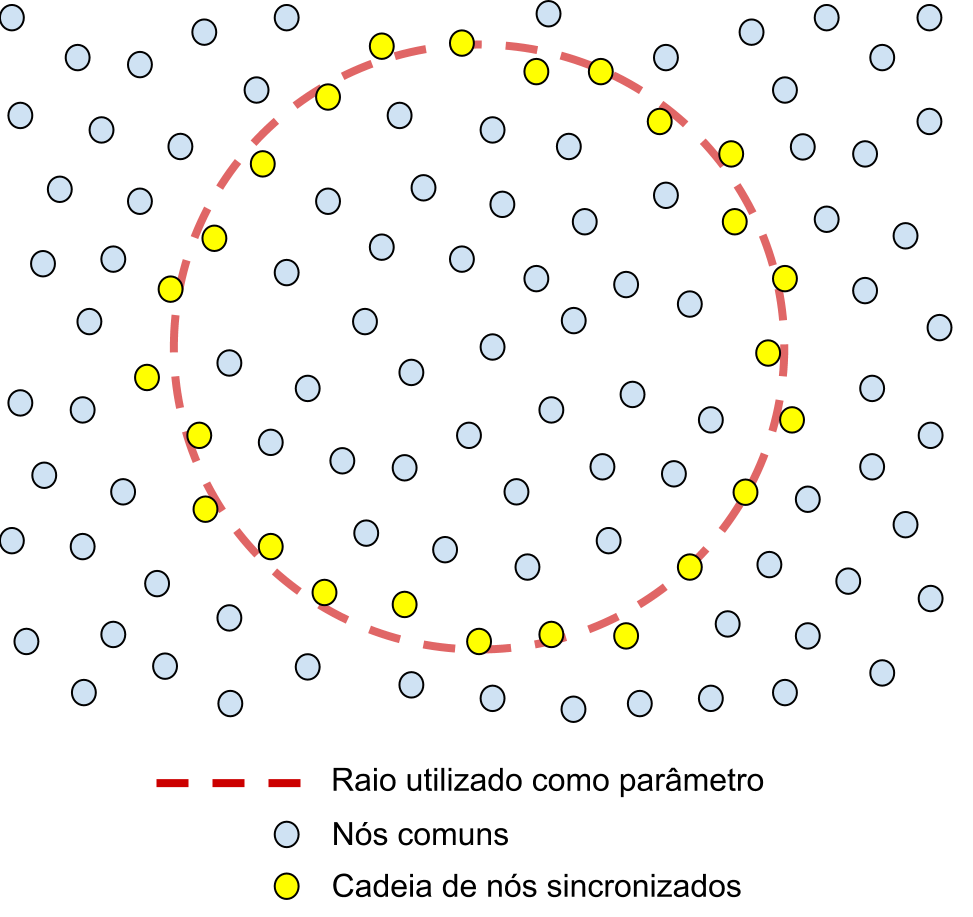
\includegraphics[width=297px,height=280px]{./Pictures/CircularBackbone.png}
% pdfLaTeX aceita figuras no formato PNG, JPG ou PDF
\caption{Cadeia de nós selecionados para sincronização.} %legenda
\label{fig:circularBackbone} %rotulo para refencia
\end{figure}

Deve-se notar que não há intervalo entre as duas transmissões. Para que isso seja possível foi determinado que cada nó siga dois cronogramas de atividades distintos sendo que o primeiro cronograma determina um período de atividade no instante $X$ e o segundo determina um período de atividade no instante $X + T_A$. Além disso, o primeiro ciclo de atividade de cada nó que participa da cadeia descrita acima deve coincidir com o segundo ciclo de atividades de seu antecessor. A Figura ~\ref{fig:backboneSynchronization} abaixo mostra como estão sincronizados os nós do exemplo anterior.

\begin{figure}[!htb]
\centering
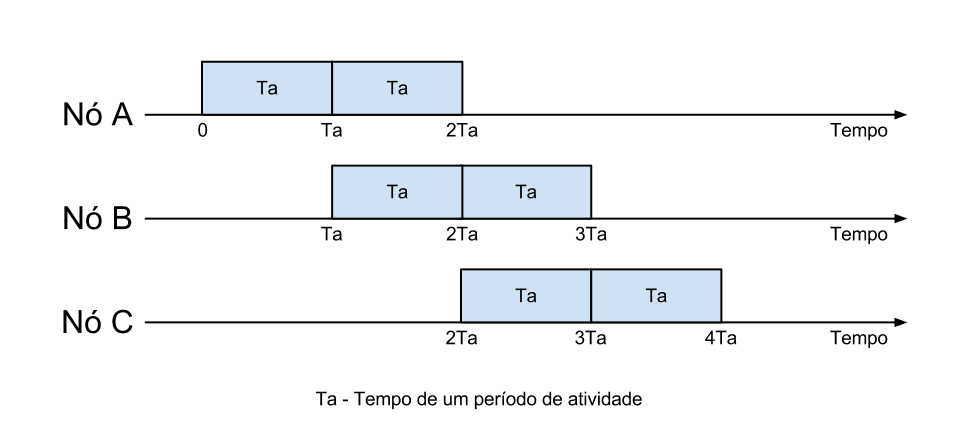
\includegraphics[width=350px,height=163px]{./Pictures/SequencialSynchronization.png}
% pdfLaTeX aceita figuras no formato PNG, JPG ou PDF
\caption{Cronogramas de atividade sincronizados sequencialmente.} %legenda
\label{fig:backboneSynchronization} %rotulo para refencia
\end{figure}

Os capítulos seguintes apresentarão uma descrição mais pormenorizada dos algoritmos utilizados para produzir a organização descrita. Ao final serão também apresentados e discutidos os resultados de simulações realizadas para avaliação dos impactos dessa organização no tempo de transmissão de pacotes entre pontos distantes na rede de sensores.

